\documentclass[tikz]{standalone}
\usetikzlibrary{positioning}

\begin{document}
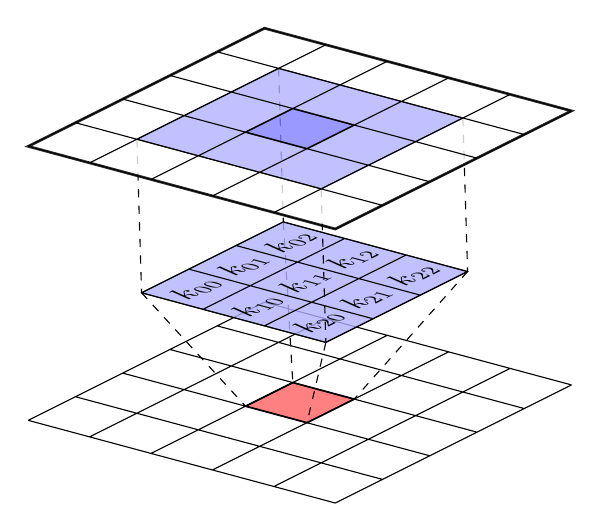
\begin{tikzpicture}[
  scale=.6,
  slanted/.style={yslant=0.5,xslant=-1.3},
  grid/.style={line width=.4pt}
]
  % Bottom layer
  \begin{scope}[yshift=-5.8cm,every node/.append style={slanted},slanted]
    \coordinate (toplayer top left) at (2,3);
    \coordinate (toplayer bottom left) at (2,2);
    \coordinate (toplayer top right) at (3,3);
    \coordinate (toplayer bottom right) at (3,2);

    % Colored cells
    \draw[fill=red!50, line width=.6pt] (2,2) rectangle (3,3);

    % Grid
    \draw[grid] (0,0) grid (5,5);
  \end{scope}

  % Middle layer
  \begin{scope}[xshift=-2mm,yshift=-2.4cm,every node/.append style={slanted},slanted]
    \coordinate (middlelayer top left) at (0,3) {};
    \coordinate (middlelayer bottom right) at (3,0) {};
    \coordinate (middlelayer bottom left) at (0,0) {};
    \coordinate (middlelayer top right) at (3,3) {};

    % Lines
    \draw[dashed] (0,0) -- (toplayer bottom left);
    \draw[dashed] (3,0) -- (toplayer bottom right);
    \draw[dashed] (3,3) -- (toplayer top right);
    \draw[dashed] (0,3) -- (toplayer top left);

    % Colored cells
    \draw[fill=blue!30,opacity=.8] (0,0) rectangle (3,3);

    % Grid
    \draw[grid] (0,0) grid (3,3);

    % Labels
    \foreach \x in {0,...,2}
      \foreach \y in {0,...,2}
        \node at (\x+.5,3-\y-.5) {\small$k_{\y\x}$};
  \end{scope}

  % Top layer
  \begin{scope}[every node/.append style={slanted},slanted]
    % Lines
    \draw[dashed] (4,1) -- (middlelayer bottom right);
    \draw[dashed] (4,4) -- (middlelayer top right);
    \draw[dashed] (1,4) -- (middlelayer top left);
    \draw[dashed] (1,1) -- (middlelayer bottom left);

    % Colored cells
    \begin{scope}[transparency group,opacity=.8]
      \draw[fill=white] (0,0) rectangle +(5,5);
      \draw[fill=blue!30,line width=.4pt] (1,1) rectangle +(3,3);
      \draw[fill=blue!50,line width=.6pt] (2,2) rectangle +(1,1);
    \end{scope}

    % Grid
    \draw[grid] (0,0) grid (5,5);
  \end{scope}
\end{tikzpicture}
\end{document}
